% !TEX TS-program = pdflatex
% !TEX encoding = UTF-8 Unicode

% Example of the Memoir class, an alternative to the default LaTeX classes such as article and book, with many added features built into the class itself.

%\documentclass[12pt,a4paper]{memoir} % for a long document
\documentclass[11pt,a4paper,article]{memoir} % for a short document
\raggedbottom
\raggedright

\usepackage[utf8]{inputenc} % set input encoding to utf8
\usepackage{graphicx}
\usepackage{amsmath}
\usepackage{caption}
\usepackage{float}
\usepackage{parskip}
\usepackage{mathpazo}
\usepackage{lscape}
\usepackage{mdwlist}
\usepackage{longtable}
\usepackage[T1]{fontenc}

\setlength{\parskip}{\baselineskip}%
\setlength{\parindent}{0pt}%

%%% PAGE DIMENSIONS
% Set up the paper to be as close as possible to both A4 & letter:
\settypeblocksize{*}{13cm}{1.8} 
\setulmargins{*}{*}{1} % 50pt upper margins
\setlrmargins{*}{*}{1}% golden ratio again for left/right margins
\setheaderspaces{*}{*}{1.618}
\checkandfixthelayout 
% This is from memman.pdf

%%% ToC (table of contents) APPEARANCE
\maxtocdepth{subsection} % include subsections
\renewcommand*{\cftappendixname}{Appendix\space}

%%% HEADERS & FOOTERS
\pagestyle{plain} % try also: empty , plain , headings , ruled , Ruled , companion

%%% CHAPTERS
\chapterstyle{section} % try also: default , section , hangnum , companion , article, demo

%%% SECTIONS
\hangsecnum % hang the section numbers into the margin to match \chapterstyle{hangnum}
\maxsecnumdepth{subsection} % number subsections

\makeatletter
\renewcommand\tableofcontents{%
\null\hfill\textbf{\huge\contentsname}\hfill\null\par
  \vspace{14pt}
  \@mkboth{\MakeUppercase\contentsname}{\MakeUppercase\contentsname}%
  \@starttoc{toc}%
}

\renewcommand\contentsname{Table of Contents}
\makeatother
\renewcommand{\baselinestretch}{1.5} 
\graphicspath{{./images/}}


%% MY COMMANDS


%% RUBRIC %%%%%%%%%%%%%%%%%%%%%%%%
% Style pointers
% > Write in the past tense
% > Passive
% > 'Each paragraph should contain a complete thought or argument'

% RUBRIC
% ---------------------------------------------------------------------------------
% Communication
% 	> Abstract
% 	> Clear statement of aims/objectives
% 	> Overall quality of report:
%		- Structure
%		- Appearance
%		- Use of English
%		- Grammar
%		- Typographical errors
%		- Nomenclature
%		- Symbols
%		- Acronyms
%		- References
% 	> Introduction to process/method
% 	> Background of industry/company context
% 	> Presentation and discussion of work and results
% 	> Conclusions and recommendations for further work
% 	> Quality of diagrams, tables
% 	> Sufficient references
% \/* "The report is well organised and well presented
% with excellent use of figures, tables and
% references. There are no spelling or grammatical
% errors. Complex information is communicated in a
% clear and logical manner." */
% \/*The purpose of the Industrial Critique report is to show that you can take an overview of a
% process, methodology or design exercise that you have personally had direct experience of, or
% been involved with, during your placement.*/
% STRUCTURE
% > Introduction
%		What DCA do, who their competitors are
%		What statistics is
%			Generic process overview
%				1. Design 2. Execute 3. Analyze 4. Present
%		Relevance of statistics to DCA
%		Outline of report structure
% > Overview of current methods
%		How DCA currently uses statistics
%			Process diagram
%			Analysis, experiment design, presentation/visualization
%			Evaluation
%		How DCA's competitors currently use statistics
%			Summary
%			Evaluation and comparison
% > Proposed alternatives
%		What methods DCA could use instead
%			Concepts
%				Analysis - Linear models (simple, multivariable, basis expansion, analysis of variance)
%				Experiment design - Blocking, factorial designs, and Taguchi
%				Data visualization - scatter and box plots, histograms
%			Implementation
%				Matlab, R, Minitab, Excel, Python
% > Conclusion

% Content
%	> Understanding of appropriate theory
%	> Understanding of process/method described
%	> Understanding of alternatives discussed
%	> Evaluation of alternatives discussed
%	> Critical discussion of work
%\/* The report is authoritative and the proposals/options
% described are suitable for implementation. An
% innovative approach is evident and there is a
% thorough awareness of the issues around
% implementation and of the economic feasibility of the
% proposals made. */
% B) How outcomes and results were checked and/or verified in DCA
% C) What went well and what did not go so well in the way statistics is done at DCA
% D) ALternative processes methods which could have been used toghther with the procs and cons of each of each of these
% E) Recommendations for improvements that could be made to the process used, giving details of the implications of these
% The focus of this critique is not on the detail of what you did or achieved but on your wider and
% deeper understanding of how the work was carried out, why it was carried out in the way it was,
% and on the alternative approaches that could have been taken. Technical detail is not a
% fundamental requirement of the critique (though should be included at an appropriate level) – it is
% the evaluation of the process/methodology that is important.

% Consider both operational and financial implications of the alternatives recommended.

% The ICR requires that you detail a critique of a process, methodology or design exercise. You are
% expected to evaluate the pros and cons of alternative approaches which may not be is use in your
% placement company and will therefore require you to carry out some research into what your
% company does and what is done elsewhere. The report must also make some recommendations,
% which may also propose further evaluation or work to implement and changes you are proposing.
% You may also need to support your conclusions and recommendations with some quantitative
% assessments of time, cost, efficiency improvements etc.

%%%%%%%%%%%%%%%%%%%%%%%%%%%%%%





%%% TITLE PAGE
\newlength\drop
\makeatletter
\newcommand*\titleM{\begingroup% Misericords, T&H p 153
\setlength\drop{0.1\textheight}
\centering
\vspace*{\drop}
{\Huge\bfseries Statistics \vspace{14pt} for \vspace{14pt}  Product Development}\\ 
\vspace{1in}
{Jerome Wynne}\\[\baselineskip]
{\scshape University of Bristol}\par
\vspace{0.61in}

%%% ABSTRACT %%
% – Set the scene (background)
% – State why the topic of your ICR is important (within the
% context of the background)
% – State why/how what was done is different or unique (or
% why it was carried out)
% – Briefly summarise results, conclusions and
% recommendations
{\bfseries Abstract}\\[\baselineskip]
{Analyzing a product's performance during development is essential to making informed design decisions, yet many engineers are uncomfortable using statistics. This shouldn't be the case: statistical tools offer a means of improving the quality and consistency of design decisions, and of developing exceptionally robust products. Here, DCA's current use of statistics is compared to modern statistical practice. Experimental, analytical, and graphical tools are suggested that would allow DCA to realize the benefits of statistical methods. }
\vfill

{\scshape \@date}\par
\endgroup}
\makeatother

% MULTILINE COMMENTS
\long\def\/*#1*/{}

%% START OF DOCUMENT
\begin{document}

\begin{titlingpage}
\titleM
\end{titlingpage}

\tableofcontents* % the asterisk means that the contents itself isn't put into the ToC
\firmlists

% List of tables/figures
\newpage
\listoftables
\listoffigures

% Notation
\newpage
\chapter*{Notation \& Glossary}
\begin{tabular} {p{2.7cm}p{10cm}}
\textbf{Attribute} & A measurable property of a \textit{unit}. \\[0.5cm]
\textbf{Block} & A set of \textit{units} thought to share some common \textit{attribute} that influences their \textit{response}. \\[0.5cm]
\textbf{Event} & A set of \textit{outcomes}.\\[0.5cm]
\textbf{Experiment$^{1}$} & The controlled collection of data. \\[0.5cm]
\textbf{Experiment$^{2}$} & Physically realizing an outcome of the system under study. \\[0.5cm]
\textbf{Factors} & \textit{Treatments} that are discrete. For example, lubricated/unlubricated.\\[0.5cm]
\textbf{Outcome} & A possible result of a \textit{trial}. \\[0.5cm]
\textbf{Probability} & A method for quantifying uncertainty, or a value representing the uncertainty of an event. \\[0.5cm]
\textbf{Response} & The measured performance of a \textit{unit}. \\[0.5cm]
\textbf{Treatment} & A modification applied to a \textit{unit}.\\[0.5cm]
\textbf{Unit} & A single test specimen - in the context of product testing, this is likely to be a prototype build of the product.
\end{tabular}

\newpage
\chapter*{\large Acknowledgements}
\vspace*{-\baselineskip}
Beyonc\'{e}, J.D.Sallinger, and Santa Claus. \\
This report would not have been possible without the encouragement of Paul Harper and technical supervision of Sophie Sladen. More broadly, I am grateful to DCA Design International for providing me a place to work on these ideas and develop professionally. Thank you to DCA's engineers - especially Will Marsh, Matthew Jones,   and Matthew Edwards - for setting the bar so high and for helping me to improve as an engineer.
\chapter*{\large Declaration}
\vspace*{-\baselineskip}
I confirm that the work presented here is wholly my own and has been generated as a result of my own thought and study. Where I have consulted the work of others it is mentioned, and where my work was part of a group effort my contribution is made clear. Where the work of another is quoted, the source is given.



%% INTRODUCTION %%
\newpage
\chapter{Introduction}
% A) Why statistics was used in DCA
DCA Design International is a 150-person product design consultancy based in Warwick. Their work is oriented towards the mechanical design of medical and consumer products. Much of what they develop are hand-held items such as insulin injector pens or deoderant cans: Figure \ref{fig:dca_profile} shows two of their most prolific designs. DCA's competitors are [DCA's COMPETITORS AND THEIR CAPABILITIES].
\par
\begin{figure}[b]

\includegraphics[width=\textwidth]{DCA_profile.pdf}
\caption{Products designed by DCA.}
\label{fig:dca_profile}
\end{figure}
\par
DCA employs about sixty mechanical engineers. Each of them are general-purpose technical consultants and experts in a particular engineering subdiscipline. DCA's substantial investment in engineering distinguishes it from other product design consultancies, many of which do not have the expertise to handle a product's technical development [REFERENCE]. This investment is manifest in both the its engineering workforce and its ownership of four test labs. 
\par
 The way in which DCA's data is collected, analyzed, and presented is the focus of this report: data-oriented activities constitute the scientific discipline of statistics. Statistical methods allow resources and information to be used efficiently, in both a mathematical sense and a practical one.
\par
Section X1 explains the company's current investigatory framework and how statistics is currently applied within it. In Section X2 the company's approach is compared to modern statistical methods, in the process of which these alternative methods are detailed and evaluated. Tools (i.e. software and tangibles) for implementing statistical methods are also discussed in the context of DCA's needs. The report concludes with an evaluation of how actionable the suggested methods are, and responds to possible criticisms of the relevance of statistics in a product design consultancy.

\newpage



%% DCA'S USE OF STATISTICS IN LAB INVESTIGATIONS %%
\chapter {Overview of DCA's Use of Statistics}
This section contextualizes DCA's uses of statistics and explains what methods are currently being applied by its engineers. The strengths and shortcomings of each method are listed, and the section closes with a summary and appraisal of DCA's approach.
\section{The Structure of a Lab Investigation in DCA}
% What does a testing sequence look like?
It's convenient to split the statistical methods that DCA apply into two factions: those brought to bear in lab investigations, and those used in other engineering activities, in particular tolerance analysis and -.
\par
A lab investigation in DCA consists of a series of experiments to understand the behaviour of a product or process. It begins with the required knowledge being identified. Experiments will then be designed, executed, and analyzed until the knowledge is acquired or is deemed no longer relevant. This process is depicted in Figure \ref{fig:investigation_diagram}.
\begin{figure}[h!]
\centering
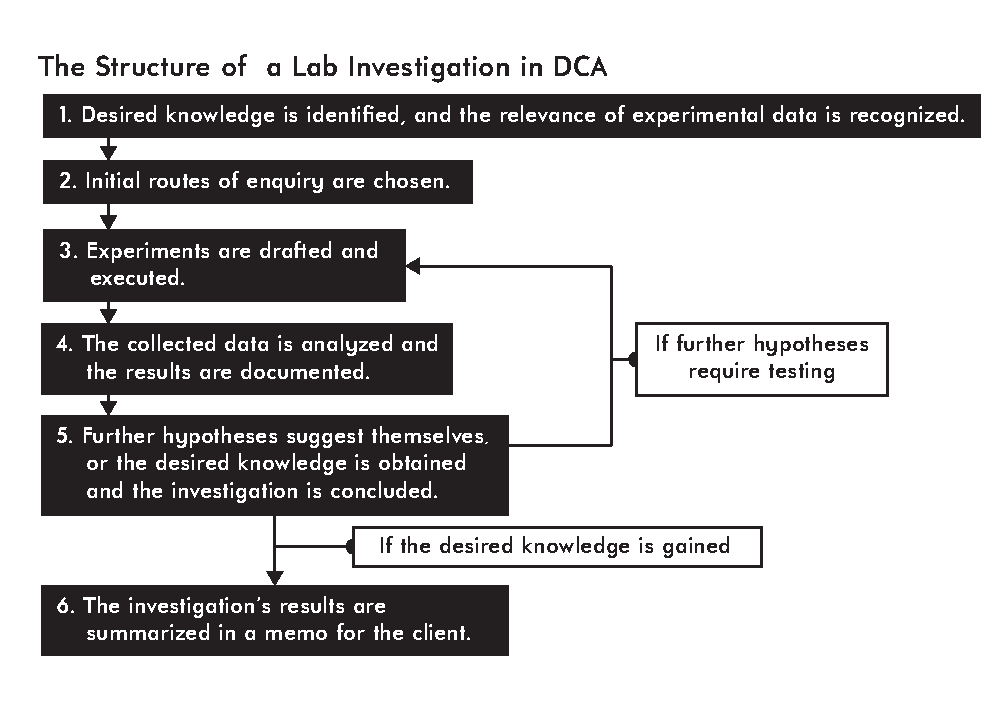
\includegraphics[width=1.2\textwidth]{Lab_Investigation_Diagram.pdf}
\caption{Investigation diagram.}
\label{fig:investigation_diagram}
\end{figure}
% What departments in DCA test their products?
All aspects of an investigation - from experiment design through to presenting the results to a client - are handled by engineers assigned to the relevant project. Typically an investigation focuses on a particular product parameter, such as the volume of fluid dispensed by an injector, or the propensity of a inhaler to fail upon being dropped. 
\par
Most lab work is conducted by engineers on medical projects.
Occasionally engineers working on fast-moving consumer goods (such as toothbrushes or lotion bottles) will run one-off tests to compare design variations or verify performance relative to some baseline. In general however, the timeframes and functional requirements of such products limit the relevance of extensive experimental investigations to them: medical products on the other hand, see a good deal of the test lab.
\par
% When do they test them and why?
As can be seen in Figure \ref{fig:time_of_tests}, the rate of testing increases as a product develops. Towards a product's relase date is when resolving minor performance issues becomes a worthwhile pursuit, exploration for future product variants become a possibility, and rehearsal for fast-approaching regulatory tests becomes essential.
\begin{figure}
\label{fig:time_of_tests}
\end{figure}
\par
% How do they test them?
DCA's engineers have access to axial and torsional testing machines, environment chambers, coordinate measuring machines, mass balances, and high-speed cameras, among other engineering instruments. Investigations commonly revolve around a particular experimental set-up, however ancillary experiments are often designed to provide supplementary information. With this in mind, it is worth noting that this report attempts to be data-agnostic in its recommendations of analytical techniques.
\par
The other engineering activities that DCA's engineers apply statistics to are tolerance analysis and, increasingly, predictive user interfaces. Before talking about this work however, DCA's use of statistics in its lab investigations will first be summarized and critiqued.

%%
\section{Experiment Design}
Experimental design and analysis can be used to make products that perform better, are more reliable, less risky to develop, and have a uniquely justifiable development process. It is expertise that would elevate DCA's capacity as a technical consultancy.
\par
Design of Experiments refers to both experiment designs and a broader philosophy of systematic experimentation. An experiment design is a particular structure of experiment, such as comparing the effects of two factors each at two levels. Good experimental design produces data that is unambiguous and relevant to the experiment's objective.
\par
Robust experiments are designed with three principles in mind:
\begin{description}
\item[Replication]{Testing a particular combination of factor levels with more than one unit. It allows experimental error to be estimated and, since unbiased errors cancel on being averaged, gives us a more precise estimate of a particular factor's influence.}
\item[Randomization]{Randomly determining the allocation of treatments to units and the sequence in which units are tested averages out the effects of nuisance variables, and validifies the assumption that obsersvations are randomly drawn from a distribution.}
\item[Blocking]{Blocking accounts for unit differences when assigning treatments - see Figure \ref{fig:blocking}. It allows the effects of a nuisance factor to be averaged out during analysis. A block is a set of similar units.}
\end{description}
These principles constitute the makings of any well-designed experiment, and they are evident in DCA's labwork: units are blocked according to factors such as component batches and time of assembly, testing and assembly sequences are randomized, and engineers fret about their sample sizes. 

\begin{figure}
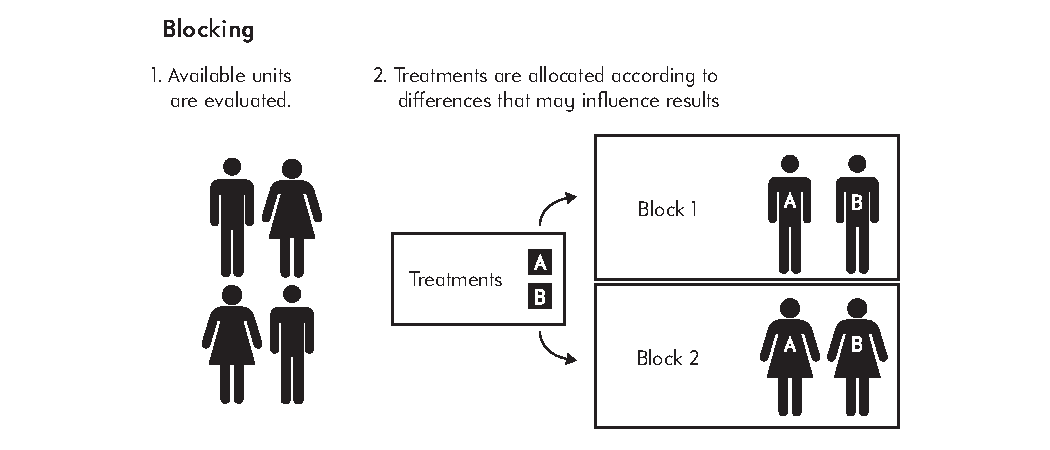
\includegraphics[width=\textwidth]{Blocking.pdf}
\caption{Diagram of what blocking involves.}
\label{fig:blocking}
\end{figure}
\par
This being said, DCA neglect pre-experimental planning and do not verify that their experimental set-ups produce repeatable results. Further, it has an inconsistent approach to screening for important factors, resulting in mired investigations. The dominant experimental strategy within the company is a best-guess approach: one factor is tested in each experiment, chosen based on the expert insight of the engineering team. Shortcomings of this method are that if the factor does not elicit the desired effect, then the next factor to vary must be guessed at, and if it is successful, then it may be tempting to stop the investigation when a better solution may be available.
\par
To systematically detail DCA's experimental procedure, it is compared against conventional experimental steps in Table \ref{tab:exp_procedure}.

\begin{landscape}
\vspace*{-3cm}
{\tiny
\begin{longtable}{p{4cm} p{7cm} p{6cm} p{6cm}}
\caption{Comparison of DCA's experimental procedure with conventional practice.}\\
\toprule[0.15em]
\textbf{Experimental step} & \textbf{DCA's implementation} & \textbf{Strengths} & \textbf{Suggestions} \\
\toprule[0.15em]
Recognition and statement of the problem. & A problem is usually identified in either other experiments or design-side activities. It is not formally stated, but is agreed in loose terms among the engineering team. There is no mechanism for assessing whether a problem is well-suited to being addressed by a lab investigation, as opposed to other analytical methods. & The benefits that experimental investigations provide, such as empirical validity and flexibility, are recognized. & A precise problem statement focuses an investigation towards a particular end, and allows progress towards this end to be gauged. It also makes it clear to the team what an investigation aims to achieve. \\ 
 &  &  & Specific problem statements make it easier to review previous work - without them, it is difficult to determine where one investigation begins and another ends. \\ 
\cmidrule{1-4}
Choice of factors, levels, and ranges. & This choice is made in engineering team meetings. Factors can be identified haphazardly: there is no labelling of those that are identified as design or nuisance factors, or whether they are controlled or uncontrolled. Ranges and levels are usually chosen according to expert knowledge. The number of levels is usually kept small (2 or 3) because differences rather than overall responses are of interest. & Level choices have a rational motivation which is justified via physical reasoning or previous experimental results. & A list of factors guides the systematic elimination of sources of variation from an experimental set-up, and can be used to survey for possible confounding factors. \\ 
 &  & Deciding which factors are relevant in a meeting uses the entire team's engineering knowledge and critical thinking skills. & A meeting should be a place to review a choice, not to generate it - conversation is not methodical and can easily miss relevant information. \\ 
\cmidrule{1-4}
Selection of the response variable. & The response variable is usually evident from the problem statement (e.g. torque output of mechanism). More than one way to measure the response variable will almost always be considered. & Engineers in the company can generate many possible response variables, and analyze their respective merits. & Precursor experiments comparing response variables may reduce the length of investigations. \\ 
 &  & The response variable chosen is chosen carefully to closely represent the system under study. & Documenting the alternative response variables would make it easier to clearly outline why one method is superior, and to transition between testing methods as circumstances change. \\ 
\cmidrule{1-4}
Choice of experimental design. & The experimental design is also chosen in a meeting. They are usually one from a small selection (detailed in the text body). The choice made is incidental, as reflected by the absence of planning documents. & Simple experiment designs are easily communicated, executed, and documented. & A well-chosen experimental design can reduce the resources (time, materials, and effort) expended in satisfying the investigation's objective. \\ 
 &  &  & Considering analysis beforehand makes it possible to ensure analytical assumptions are met. \\ 
\cmidrule{1-4}
Performing the experiment. & Engineers run their experiments in a laboratory. Frequently run experiments have protocols; hand-written observations are mandated for all experiments. & Labs afford flexibility in the level of experimental control. & Experimental fixtures should be shown to generate repeatable, reliable results before being used. \\ 
 &  & Blank observation sheets encourage critical thinking about the experiment & Images of test set-up would make it much easier to retrospectively understand an experiment. \\ 
 &  & Experiments are run by engineers solving the problem - this makes engineers personally responsible for their results, and exposes them to undocumented experimental information. & Observation sheets could provide guidance on what factors to monitor. \\ 
\cline{1-4}
Analysis of the data collected. & Analyses are run as soon as data is available, and will be handled by the engineer that ran the experiment. Excel - and occasionally Matlab - is used. The conclusions tend to be judgemental as opposed to statistical. Compared to the time spent running the experiment, analysis is brief. Analysis is discussed in more detail in the next section. & Engineering expertise is applied to explain experimental results in a physically meaningful way. & Statistics should be used to ensure that sound conclusions are made - subjective assessment alone is susceptible to various biases that can lead to lost time and confusion. \\ 
 &  &  & Time invested in analyses should be seen as what makes an experiment practically useful, rather than a formality between experiments. \\ 
\cmidrule{1-4}
Conclusions and recommendations & Conclusions are incorporated into client memos and presentations. Interim results are presented at internal meetings - graphics play an important role in communicating results. & The importance of graphics is realized and put to good effect in client presentations. & Charts exist beyond those being used that may make it easier to demonstrate experimental results. \\ 
 &  & Conclusions are presented in a way that is accessible and avoids needless technicalities. & Experimental results are not supplemented by estimates of uncertainty. \\ 
\bottomrule
\label{tab:exp_procedure}
\end{longtable}
}
\end{landscape}


\par
The experimental designs used in the company are enumerated, explained, and critiqued in Table \ref{tab:exp_designs}.
\renewcommand\arraystretch{1.5}
\begin{table}[H]
\hspace*{-2.25cm}
\small
\centering
	\begin{tabular}{p{3.5cm} p{6cm} p{6.5cm}}
	\toprule
	\textbf{Experimental Design} 		& 	\textbf{Description}	&	\textbf{Evaluation} \\\toprule
	Randomized complete block design	 & 	Each treatment is randomly assigned to at least one unit from every block. &  Allows the effects of nuisance variables to be eliminated during analysis, provided the block factor and treatment do not interact. \\
	& & Lends itself to established analytical techniques (e.g. ANOVA). \\
	& & Can be extended to block on more than one factor (such a design is called a Latin square) \\
	& & Not possible if the number of units in a block is fewer than the number of treatments to be tested. \\
	&&\\
	Factorial design & Applied to experiments in which more than one factor is varied - all combinations of factor levels are tested. & More time-efficient than testing one factor per experiment. \\
	& &  May be limited by resources if there are many factors \\
	& & Allows interaction effects to be estimated.
	\\\bottomrule
	\end{tabular}
	\hspace*{-2.25cm}
	\caption{Experimental designs applied in DCA.}
	\label{tab:exp_designs}
\end{table}

\newpage
%%
\section{Analysis of Experimental Data}
This section provides a short overview of the statistical tools applied to experimental data in DCA: the content of several hundred test reports was tabulated to inform this discussion, which focuses on summary statistics and interval estimates.
\par
Analyses in DCA were found to rely heavily on expert knowledge of the systems being tested and rarely on statistical results. This is probably because the relevance of statistics may not be clear, and how it might be applied even less so. Which is understandable - it's widely agreed that most people's experience with statistics is one of discomfort and bemusement. Having said this, relying on intuition alone risks falling prey to cognitive biases, missing valuable information that isn't superficially obvious, and being unable to properly relate physical behaviours to experimental observations. Foregoing statistics when analyzing product behaviour severely handicaps the ability of an engineer to design a robust product.
\par
Many of the reports surveyed contained summary statistics, such as arithmetic means, variances, maximums, minimums, and so on. A few made use of interval estimates as informed by a regulatory standard, and one report applied a t-test.
\par
\subsection*{Summary Statistics}
 A summary statistic is a value describes an aspect of a random variable's distribution. A random variable (r.v.) is a function that maps events onto real numbers. For example, we could define an r.v. $X$ that maps the outcomes of a coin toss onto the numbers 1 and 0:
 \begin{align}
	X(\texttt{Coin lands Heads}) = 1 \\
	X(\texttt{Coin lands Tails}) =0
 \end{align}
Usually the choice of mapping is quite natural - for example, we might use an r.v. that counts the number of sucesses in many trials, or that takes on the value of a measurement.
\par
Variation in the events that an r.v. maps from is described using a probability distribution. Each value is weighted according to its probability or, in the case of continuous-valued r.v.s, its contribution per unit length to the cumulative probability. Figure \ref{fig:example_pd} highlights this difference.
\par
The essential problem of experimental statistics is understanding the behaviour of a broader population from just a sample. In product design, this means using measurements from a limited number of prototypes to estimate the variation in a much larger population of units. The attributes of this variation - such as its spread and average - can be estimated using summary statistics.
 \par
A mean of several independent measurements, for example, approximates the mean of the underlying population's distribution. The accuracy of this estimate improves as more samples are tested, with diminishing returns, a relationship that is shown in Figure \ref{fig:se_with_sample_size}. This estimate's average difference to the true mean is called the standard error, and it corresponds to $\frac{\sigma}{\sqrt{n}}$, where $\sigma$ is the standard deviation of the population and $n$ is number of units in the sample. DCA implicitly appeal to this relationship when they choose to run more units in a test, although it did not seem to be used actively to gauge appropriate sample sizes.

Certain summary statistics can be thought of as estimates of a distribution's parameters. These are values that constrain a particular distribution's shape. The normal distribution's shape, for example, can be specified by supplying just two values: the variance (spread) and mean (location). Viewing statistics as an exercise in estimating a distribution's parameters will be seen again later, in the section on Bayesian inference.

\begin{figure}
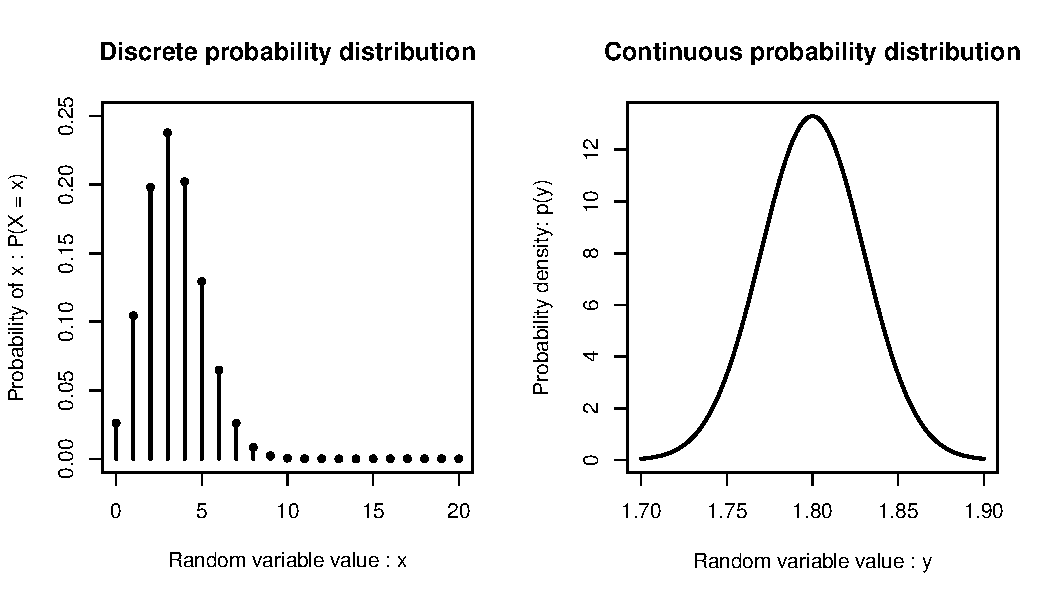
\includegraphics[width=\textwidth]{probability_distributions.pdf}
\caption{Left: Probability mass function. Right: Probability density function.}
\label{fig:example_pd}
\end{figure}
\begin{figure}
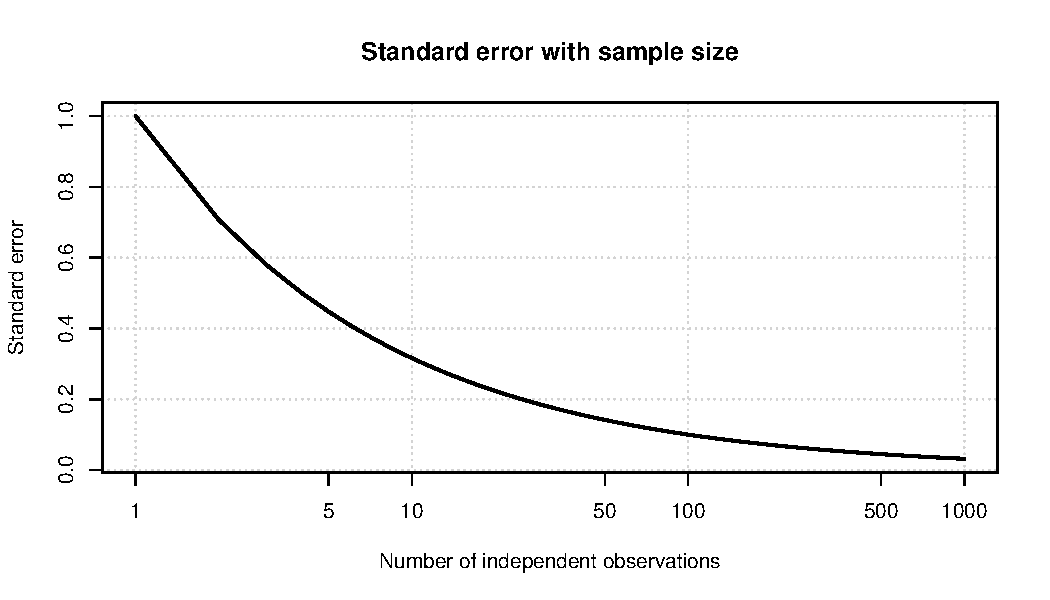
\includegraphics[width=\textwidth]{se_with_sample_size.pdf}
\caption{Convergence of sample mean to population mean.}
\label{fig:se_with_sample_size}
\end{figure}
\par

\newpage
\subsection*{Tolerance Intervals}
DCA's most sophisticated statistical analysis is based on ISO 16269-6, \emph{Determination of statistical tolerance intervals}. This standard outlines how to construct tolerance intervals under either no assumptions about the random variable's distribution, or the assumption that the random variable has a normal distribution. A tolerance interval is a range of values that contain a particular fraction of the population to a given confidence level; a confidence level is the proportion of intervals constructed that will contain that fraction of the population. So tolerance intervals allow us to make statements about the performance of a population, with clear limits on that statement's uncertainty. A derivation of a one-sided interval is given in Appendix A, and can be summarized as:
\begin{enumerate}
	\item Defining $k$ such that
		\begin{equation}
			P(\bar{x} + ks \geq \mu + u_p \sigma) = 1 - \alpha
			\label{eq:tol_interval}
		\end{equation}
	Where $\bar{x}$ is the sample mean, $s$ is the sample standard deviation, $\mu$ is the true mean of the population, $\sigma$ is its true standard deviation, and $u_p$ is such that $\mu + u_p\sigma$ is greater than $p\%$ of the population. $\alpha$ is the confidence level. \newline In words, $k$ is such that $\bar{x} + ks$ will  be greater than the $p\%$ of the population $(1 - \alpha)\%$ of the time.
	\item If $x$ is assumed to have a normal distribution then $u_p$ can be read off a table of normal values, and by definition $\frac{(n-1)s^2}{\sigma^2}$ will have a chi-square distribution (see Appendix A). What this means is that $k$ has the same distribution as a $t$-distributed r.v. centered at $\sqrt{n}u_p$ and scaled by $\frac{1}{\sqrt{n}}$:
		\begin{equation}
			k = \frac{1}{\sqrt{n}}t_{n - 1}(\sqrt{n}u_p) 
		\end{equation}
	\item  Bonanza! The lower interval containing at least $95\%$  of the population is
\begin{equation}
	\Big(-\infty, \bar{x} + \frac{t_{1 - \alpha}(\sqrt{n}u_p, n - 1)\cdot s}{\sqrt{n}}\Big]
\end{equation}
A fraction $1 - \alpha$ of these intervals will contain less than $p\%$ of the population, as shown in Figure \ref{fig:tolerance_intervals}.
\end{enumerate}

\begin{figure}[H]
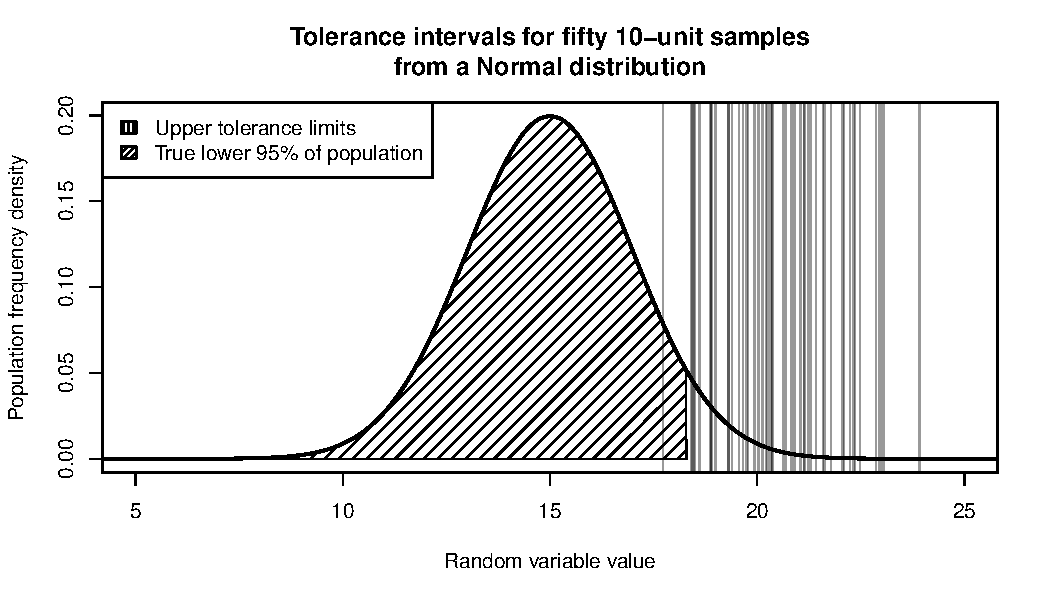
\includegraphics[width=\textwidth]{tolerance_intervals.pdf}
\caption{Twenty tolerance limits versus population limit.}
\label{fig:tolerance_intervals}
\end{figure}
The strengths and suggestions for DCA's tolerance intervals are listed in Table \ref{tab:tol_intervals}.
\begin{table}[b]
\caption{Evaluation of tolerance intervals.}
\small
\hspace*{-.5cm}
\begin{tabular}{p{6.5cm}p{6.5cm}}
\toprule
\textbf{Strengths}	&	\textbf{Shortcomings} \\
\toprule
Provides a threshold indicating roughly where a certain fraction of the population is. & Can be misinterpreted as specifying the probability that a constructed interval contains at least $95\%$ of the population. \\
Plug-and-play & Normality assumption needs checking \\
 & Repeated use at a low confidence level increases the probability that the limit will be under-estimated. \\
\bottomrule
\end{tabular}
\label{tab:tol_intervals}
\end{table}

\newpage
% Confidence intervals
\subsection*{Confidence Intervals}
Another tool that DCA's engineers occasionally use is confidence intervals, which indicate a range of values that a population parameter is likely to fall within. This range will only contain the population parameter a certain fraction of the time however, a problem that's unavoidable since there will always be a chance that an unrepresentative sample is drawn. For example, if we were to construct a confidence interval for the population mean of 100 samples, each of 5 units, the confidence level would tell us how many of these intervals would - on average - contain the actual value of the population mean. Figure \ref{fig:confidence_intervals} demonstrates this idea. Confidence intervals can be placed on any parameter estimate, although they're usually used to quantify the uncertainty on a mean. Their derivation is similar to a tolerance interval's: the two-sided one is as follows:
\begin{align}
	\text{P}(\bar{x} - ks \leq \mu \leq \bar{x} + ks) &= 1 - 2\cdot \text{P}(\bar{x} - ks \leq \mu) = 1 - \alpha \nonumber\\
	\implies \frac{\alpha}{2} &= \text{P}(\frac{\bar{x} - \mu}{s} \leq k) 
\end{align}
The last line implies that $k$ has a $t$-distribution with $n - 1$ degrees of freedom, so that the confidence limit that contains the true mean $(1 - \alpha)\%$ of the time is
\begin{equation}
	[\bar{x} - t_{n-1}(\alpha)\cdot s, \ \bar{x} + t_{n-1}(\alpha)\cdot s]
\end{equation}
\begin{figure}[H]
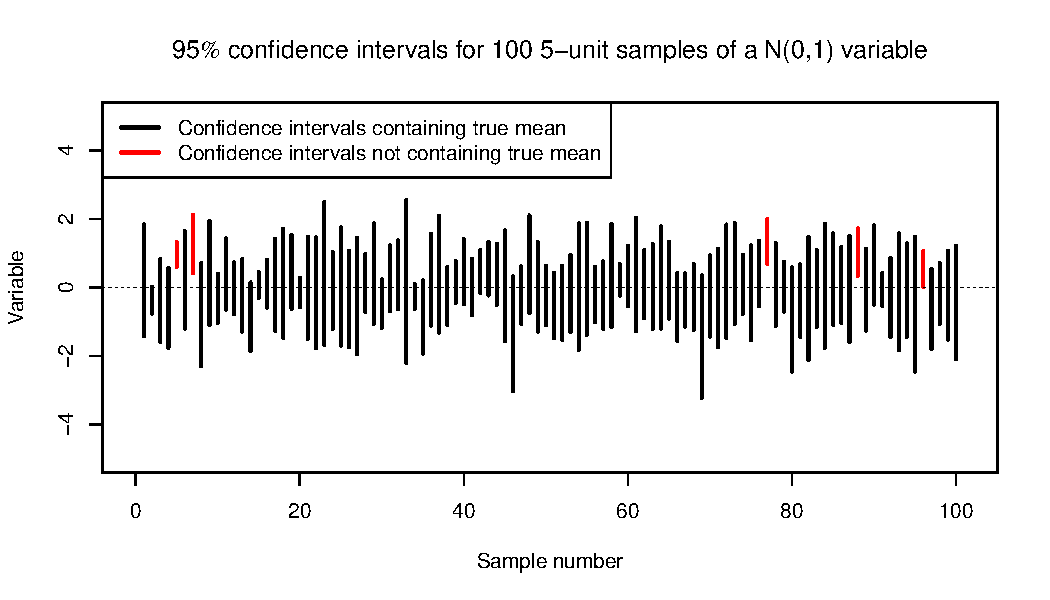
\includegraphics[width=\textwidth]{confidence_intervals.pdf}
\caption{}
\label{fig:confidence_intervals}
\end{figure}

\newpage
\subsection*{Monte Carlo Simulation}
Monte Carlo simulation approximates a quantity by simulating the random process generating it . In DCA it's been used to analze tolerance chains in products. The use case was somewhat similar to the following: the 95th percentile of some analytically inconvenient combination of distributions, each corresponding to a part dimension, was needed. Take $Y \sim \text{Binom}(n = 10, p = X)$ as an example, where $X \sim \text{Beta}(a = 7, b = 3)$\footnote{The beta distribution is a continuous and generates a number between $0$ and $1$, which makes it useful in modelling the distribution of a probability.}. Rather than attempt to derive the distribution of this dimension's value directly, tens of thousands of values of $y$ were first generated according to $Y$'s distribution using a computer. Each of these values were then used to generate a value of $x$ from $\text{Binom}(n = 10, p = y)$. The resulting frequencies of the $x$ values then represented the dimension's distribution. It was then possible to calculate the mean by averaging over all the $x$ values obtained. A diagram of this process is shown in Figure \ref{fig:monte_carlo}.
\begin{figure}[b!]
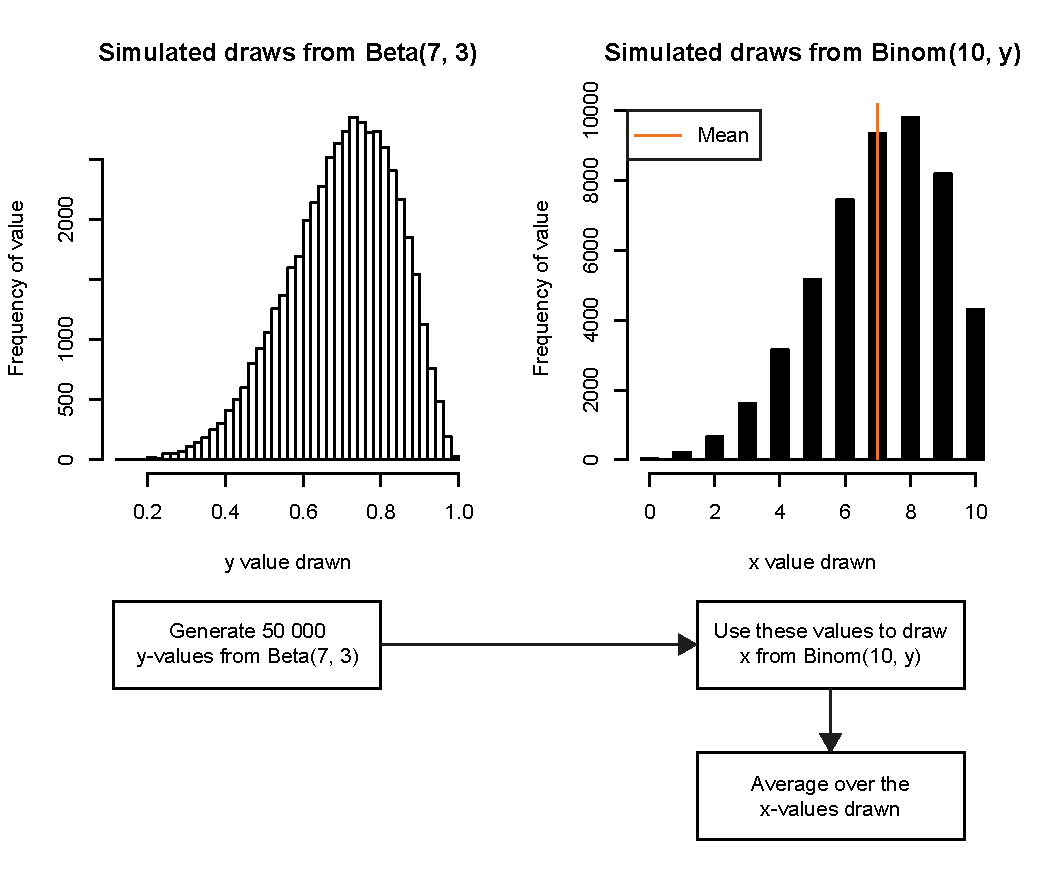
\includegraphics[width=0.87\textwidth]{monte_carlo_simulation.pdf}
\caption{Process diagram for a Monte Carlo simulation.}
\label{fig:monte_carlo}
\end{figure}


\newpage
\section{Visualizing Experimental Data}
Visualization is essential to clearly and convincingly summarizing an experiment's results. Graphical tools allow engineers and clients to see for themselves what's been discovered. A plot should relevant, easily interpretable, and accurately convey its underlying data.
\par
DCA's reports and client presentations frequently contain plots of the data collected from an experiment, typically generated using either Microsoft Excel or Matlab. The plots used are line and bar charts, along with the occasional scatterplot.
\par
Line charts are particularly ubiquitous in DCA because they're directly plottable from the raw data provided by axial and torsional testing machines. As a consequence of this many graphical summaries are usually overlaid line plots, similar to that shown in Figure \ref{fig:line_plots}. The effectiveness of this use-case is evaluated in Table \ref{tab:line_chart}: in short, this type of plot can include a lot of redundant information and can make it difficult to see how individual units are behaving.
\par
Bar charts are also used fairly frequently to display performance relative to a nominal value, and a particular format of scatterplot is used to present the results of a tolerance limit analysis. The latter is shown in Figure \ref{fig:tolerance_intervals_plot}. 
\begin{table}[h!]
\caption{Evaluation of the line chart.}
\small
\hspace*{-.5cm}
\begin{tabular}{p{6.5cm}p{6.5cm}}
\toprule
\textbf{Strengths}	&	\textbf{Shortcomings} \\
\toprule
Allows an entire test to be viewed simultaneously, providing a high-level summary of results.	&	May provide irrelevant information - it's often the case that only the peak or average values are of interest	\\
Is easily relatable to physical observations during a test.	&	Directs focus to extremes of group ranges, rather than the distribution of each group's performance.	\\
Its meaning can be understood without explanation - it is a universally familiar chart.	&  Obfuscates data artifacts that aren't related to location or dispersion (such as harmonic content). \\
&  Can obscure the behaviour of individual units. 			\\
\bottomrule
\end{tabular}
\label{tab:line_chart}
\end{table}

\begin{figure}
	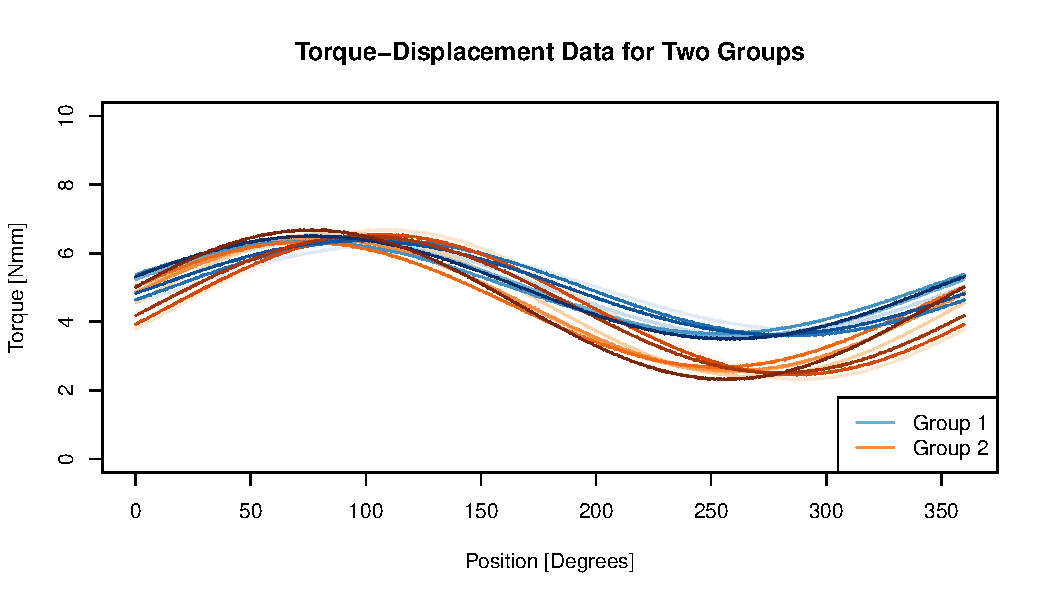
\includegraphics[width=\textwidth]{overlaid_line_chart.pdf}
	\caption{Sample summary line chart from a DCA test report.}
	\label{fig:line_plots}
\end{figure}
\begin{figure}
	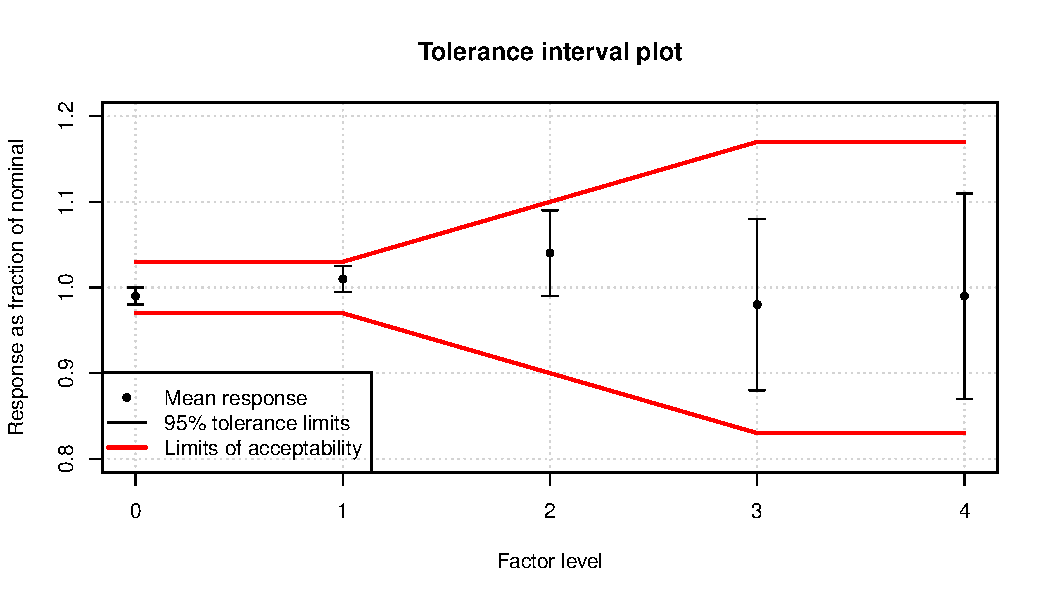
\includegraphics[width=\textwidth]{tolerance_intervals_plot.pdf}
	\caption{Tolerance interval plot.}
	\label{fig:tolerance_intervals_plot}
\end{figure}

%%  SUGGESTED METHODS %%
\chapter{Suggested Methods}\label{suggested_methods}
\section{Experiment design}
\subsection*{Experimental pre-planning}
\subsection*{Fractional factorial designs}
\subsection*{Taguchi designs}

\section{Analysis}
\subsection*{Linear Models}
% What's a regression model?
% How's it useful to DCA?
% What do they consist of?
% What are their limitations, and how can they be applied to more difficult problems?
Typically a test can be viewed in terms of input and reponse variables: in a tensile test of a unit for instance, load might be viewed as the reponse and displacement as a predictor. Linear models describe a response as a linear function of some parameters $\beta$, each weighted by possible predictors. An example of such a model would be:
\begin{equation}
	f(x_1, x_2) = \beta_0 + \beta_1 \cdot x_1 + \beta_2 \cdot e^{x_1}+ \beta_3 \cdot x_1 \cdot x_2
\end{equation}
Where  $x_i$ is a measured quantity, $\beta_j$ is the coefficient of the $j$th term, and $f$ is the model to be fit. Note that while the coefficients $\beta_i$ are linear, the predictors can be any kind of function of the measurements. Fitting this model such that $f(x)$ tends to be close to $y$ adjusts the coefficients to reflect their predictors' influence on the response. A common type of fit is a simple linear fit:
\begin{equation}
	f(x_1) = \beta_0 + \beta_1 \cdot x_1
\end{equation}
This can be extended to more than one variable, where it becomes known as multiple linear regression:
\begin{equation}
	f(x_1, x_2) = \beta_0 + \beta_1 \cdot x_1 + \beta_2 \cdot x_2
\end{equation}
Linear regression of a dummy dataset onto one and two predictor variables is shown in Figure \ref{fig:linear_regression}. 
\begin{figure}
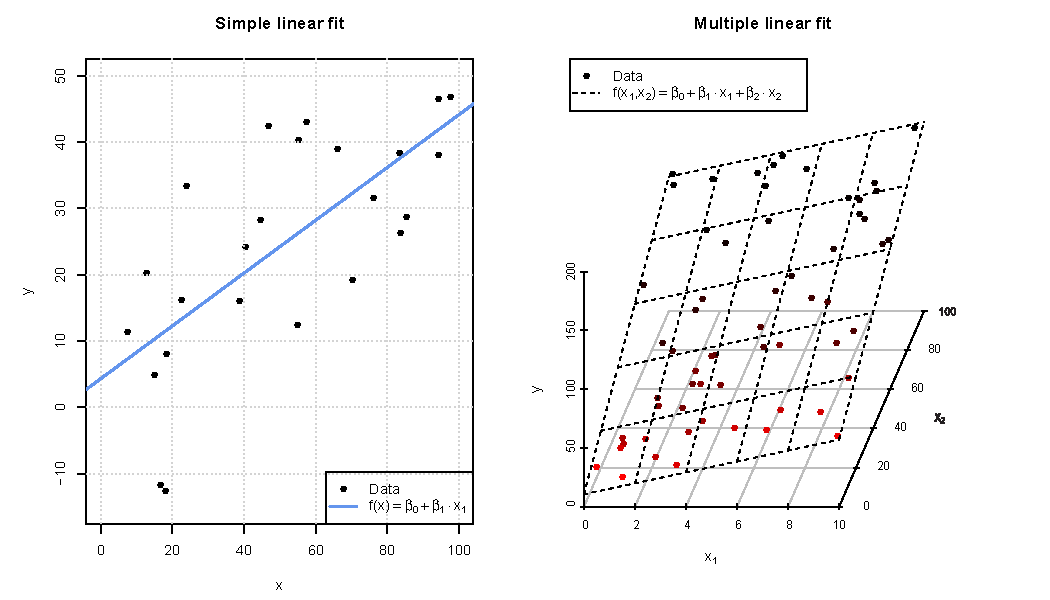
\includegraphics[width=\textwidth]{linear_fits.pdf}
\caption{Linear fits}
\label{fig:linear_regression}
\end{figure}


\newpage
\subsection*{Bayesian Inference}
% What is Bayesian inference?
% How can it be useful to DCA?
% What does it consist of?
% How does it relate to other statistical methods, what are its limitations, and how can it be used for more difficult problems?
Summary statistics state what the most likely value for a parameter\footnote{Reminder: a parameter is a number that controls the shape of a distribution.} is, based on the data alone. They don't say how much more likely this value is is than other values, or let knowledge besides the data be included.
\par
 In reality, a sample will suggest a distribution of plausible values, and there will be expert knowledge that can be used. Bayesian inference combines this knowledge with the collected data to estimate a distribution of possible parameter values. Figure \ref{fig:annotated_posterior} points out the benefits of determining how probable particular parameter values are, compared to the point estimates provided by summary statistics.
\begin{figure}[b]
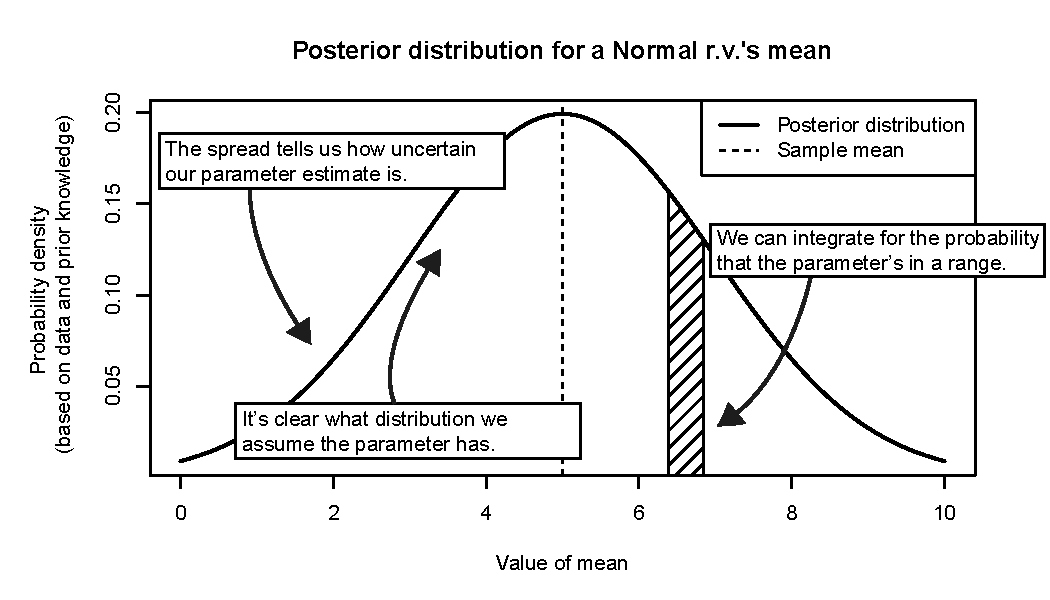
\includegraphics[width=\textwidth]{annotated_posterior.pdf}
\caption{An annotated posterior distribution.}
\label{fig:annotated_posterior}
\end{figure}
\par
Bayesian methods would be useful to DCA because they're more easily understood, visualized, and explained than classical methods, and are relevant to a broader range of situations. They also allow expert knowledge to be used, making it possible to reach a sanitary comprimise between gut-feel and experimental observation. These claims will can be explained and justified in the context of an example.
\par
The proportion of units passing a specification test is a useful measure of a design's suitability for the problem at hand. Using the results from a test sample and the expertise of an engineering team, it's possible to estimate what pass rates would be likely if the design were to be produced in larger volumes by a similar method.
\par
Say that a sample of $n$ units are tested, and $n$ pass. The engineering team also collude to produce a distribution for the passing rate $\theta$ that's tall near values they think probable and shallow near ones that seem unlikely. The team's aim is then to calculate the probability of a unit passing, given their data and preliminary estimates: Bayes' theorem can be used to do this.
\begin{equation}
  p(\theta|y) = \frac{p(y|\theta)\cdot p(\theta)}{\int_{\theta}p(y|\theta)\cdot p(\theta)\cdot d\theta}
  \label{eq:bayes}
\end{equation}
Expression (\ref{eq:bayes}) means that a passing proportion is more probable if it makes the number of units seen to pass more likely and seems sensible to the engineering team. The denominator of this expression is constant w.r.t. $\theta$, so that
\begin{align}
  p(\theta|y) &\propto p(y | \theta)\cdot p(\theta)   \label{eq:unnorm_bay} \\
  \small{\texttt{Posterior}} &\propto\small{{\texttt{Likelihood} \cdot \texttt{Prior}}} \nonumber
\end{align}
(\ref{eq:unnorm_bay}) makes it clear that to estimate $p(\theta|y)$, two things are needed:
\begin{itemize}
\item The probability of the data assuming a particular passing proportion, $p(y|\theta)$ (the \emph{likelihood}).
\item  The probability of a passing proportion according to the engineerig team, $p(\theta)$ (the \emph{prior}).
\end{itemize}
The likelihood is the probability of $y$ units passing and $(n-y)$ units failing. Assuming that passes and failures and independent and the units come from populations with the same underlying passing probability, then the probability of $y$ passes given that $\theta$ of that population would pass is:
\begin{gather}
  p(y|\theta) = \binom{n}{y} \theta^y (1 - \theta)^{n - y}
  \label{eq:binom_likelihood}
\end{gather}
The prior distribution, $p(\theta)$, encodes knowledge of what passing proportions are probable. If the engineering team is unsure what the passing proportion would be, then they may assume that all values are equally likely:
\begin{equation}
  p(\theta) = 1 \quad \theta \in [0, 1]
  \label{eq:unif_prior}
\end{equation}
Figure \ref{fig:binom_bayes_inference} displays the prior and likelihood distributions. At this point it's possible to do one of two things: the posterior can either be evaluated analytically, or it can be computed. Irrespective of the method chosen, the expression being evaluated is:
\begin{equation}
	p(\theta|y) = \texttt{constant}\cdot p(y|\theta) \cdot p(\theta)
	\label{eq:example_bayes}
\end{equation}
In practice, (\ref{eq:example_bayes}) is calculated using a computer. A grid of $\theta$ values is defined, and their prior probabilities and likelihoods are calculated in line with the functions in (\ref{eq:unif_prior}) and (\ref{eq:binom_likelihood}). This process can be described by the pseudocode:
\begin{align}
  \quad n &:= \small{\texttt{No. of units tested}} \\
   \quad y &:= \small{\texttt{No. of units that passed}} \\
  \boldsymbol{\theta} & := (0, \ 0.01, \ \dots, \ 1) \\
  \small{\texttt{Prior}} &:= \small{\texttt{Uniform}}(\boldsymbol{\theta}, [0, 1]) \\
  \small{\texttt{Likelihood}} &:= \small{\texttt{Binomial}}(y, n, \boldsymbol{\theta}) \\ 
  \small{\texttt{Posterior}} &:= \small{\texttt{Prior} \odot \texttt{Likelihood}}
\end{align}
Where $\texttt{Uniform}$ returns the probability density of the uniform distribution for each value in $\boldsymbol{\theta}$ (i.e. a list of ones), $\texttt{Binomial}$ returns the probability of $y$ in $n$ units passing given each of the passing probabilities in $\boldsymbol{\theta}$, and $\odot$ is the element-wise product.
The posterior list would contain the probability density for each passing proportion $\theta$, and is again shown in Figure \ref{fig:binom_bayes_inference}. The pointy part indicates more probable values - a taller, pointier peak represents a more certain estimate because a few values have a much higher probability than lots of others. In the same spirit, the flat prior that was used can be understood as highly uncertain.
\begin{figure}
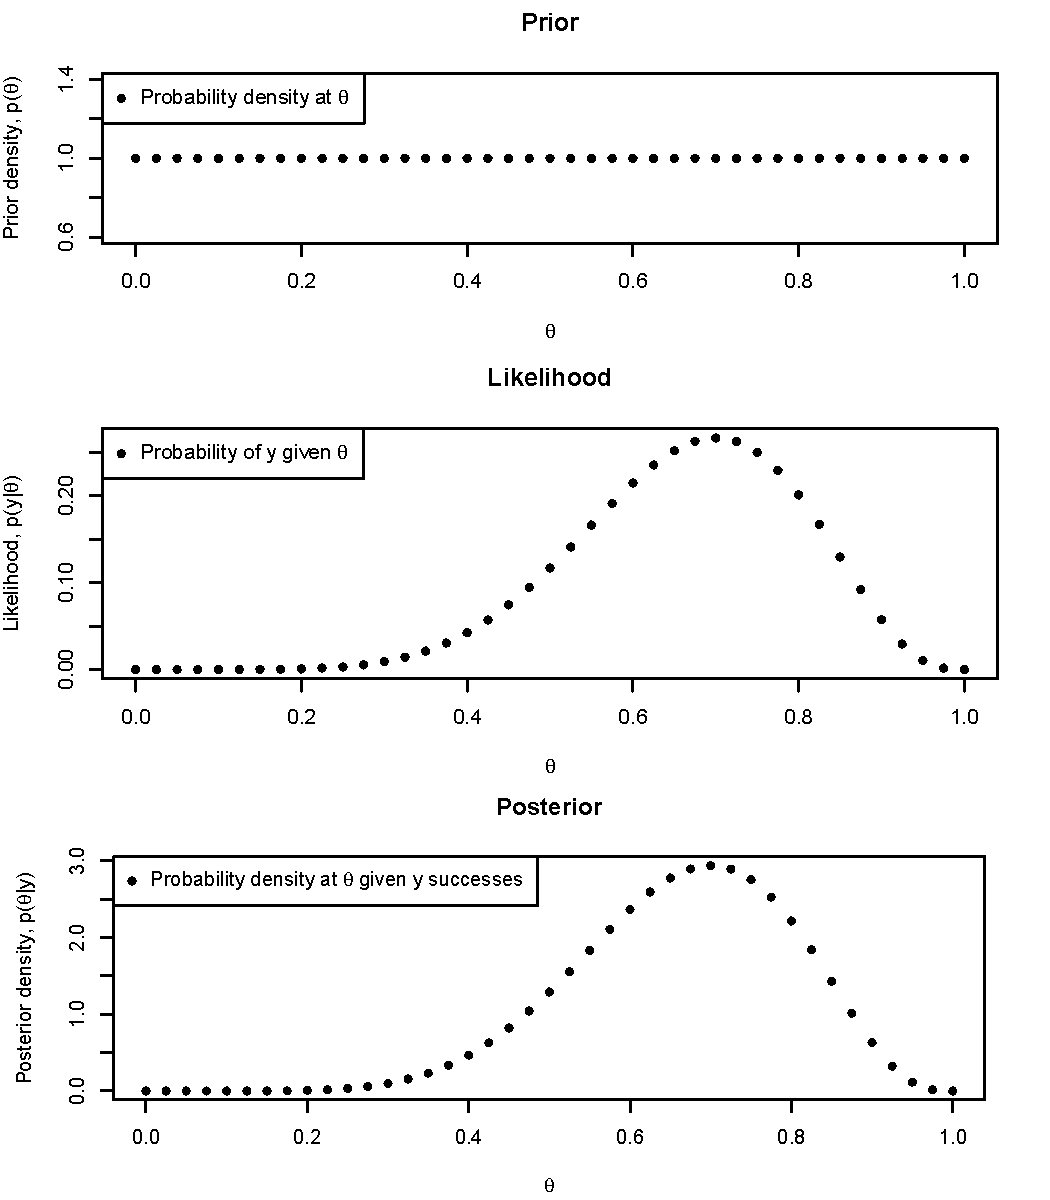
\includegraphics[width=\textwidth]{Bayesian_inference.pdf}
\caption{}
\label{fig:binom_bayes_inference}
\end{figure}
\par
One of the neat things about Bayesian inference is that the posterior of one analysis can be used as the prior of the next: this means that the information from tests is able to accumulate. This idea is shown in Figure \ref{fig:updating_posterior.pdf} - the flat prior represents initial ignorance about whether a unit will pass: as more units are run, an increasingly narrow peak forms around the most probable passing probability.
\begin{figure}
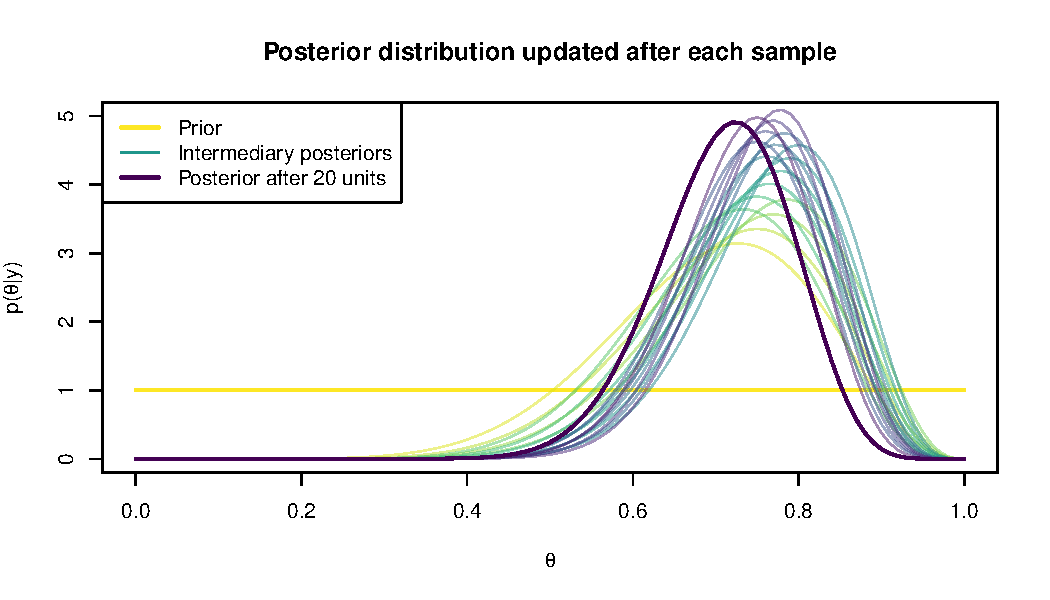
\includegraphics[width=\textwidth]{updating_posterior.pdf}
\label{fig:updating_posterior}
\caption{The uncertainty in the posterior decreases as more samples are conditioned upon.}
\end{figure}
\par
Once the posterior has been calculated, it can be used to predict the behaviour of future units. $\tilde{y}$ denotes the number of future units that pass, $\tilde{n}$ is the number of units tested. The probability of $\tilde{y}$ successes, based on the observed data and additional information, is the weighted average of $\tilde{y}$ successes over all possible values of $\theta$:
\begin{equation}
	p(\tilde{y}|y) = \int_{\theta}p(\tilde{y}|\theta, y)\cdot p(\theta|y) \cdot d\theta
\end{equation}
Once again, we can avoid some potentially mischievous mathematics by approximating this integral using a computer: draw samples of $\theta$ based on $p(\theta|y)$, then sample a value of $\tilde{y}$ from $p(\tilde{y}|\theta, y)$. Do this many times and the relative frequency of $\tilde{y}$ values will tend towards $p(\tilde{y}|y)$.
\begin{align}
\small{\texttt{for (i in [1, 10 000]) \{}} &\\
	\tilde{n} &:= \small{\texttt{No. future units to be tested}} \\
	\boldsymbol{\tilde{y}} &:= (0, 1, \dots, \tilde{n}) \\
	\theta &:= \small{\texttt{Sample(}}\boldsymbol{\theta}\small{\texttt{, Posterior)}} \\
	\small{\texttt{Posterior predictive[i]}} &:= \small{\texttt{Sample(}}\boldsymbol{\tilde{y}}\small{\texttt{, Binomial(}}\tilde{y}, \tilde{n}, \theta\small{\texttt{))}}\\
	&\quad\quad \small{\texttt{ \} }}
\end{align}
Figure \ref{fig:posterior_predictive} shows a plot of this posterior predictive distribution, along with the $5\%$ lower limit on the number of units that will pass. This limit can be interpreted as a bound on the plausible number of units to pass, according to the weighted evidence, or it can be given a frequency interpretation: if we were to run 20 samples of 100 units, we would expect one of these samples to have a pass rate of less than 54 units.
\begin{figure}
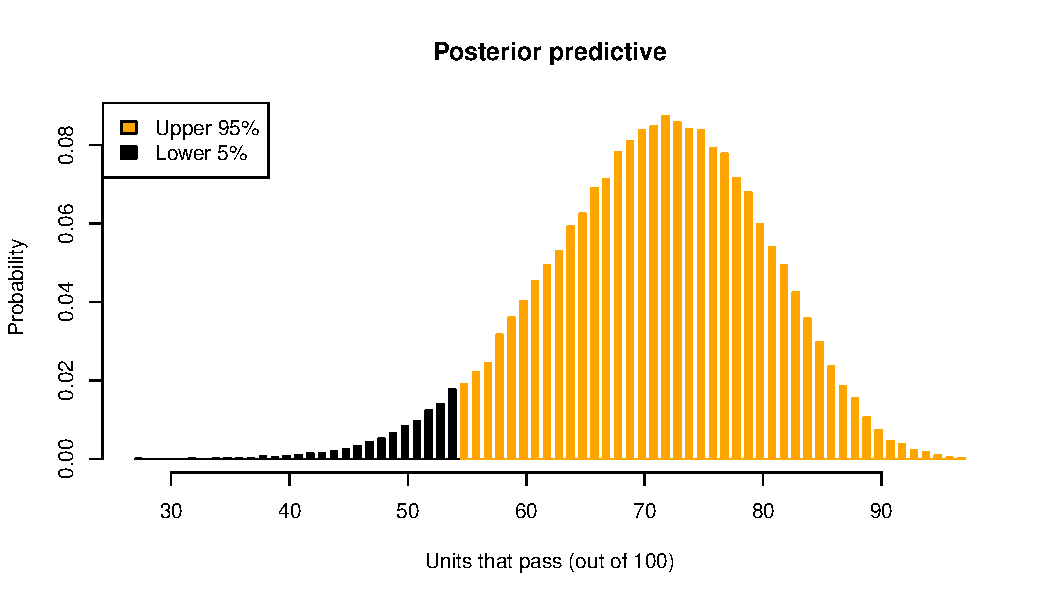
\includegraphics[width=\textwidth]{posterior_predictive.pdf}
\caption{Posterior predictive distribution for the number of passing units in a 100-unit run.}
\label{fig:posterior_predictive}
\end{figure}
Another advantage of Bayesian methods over hypothesis testing is that it's relatively easy to build models that estimate many parameters simultaneously. An instance of this might be when estimating the mean and variance of data that's assumed to have a normal distribution. The only change relative to the single-parameter scenario is that we need to define the prior and likelihood in Equation \ref{eq:unnorm_bay} over two parameters instead of one:
\begin{equation}
	p(\theta_1, \theta_2 | y) \propto p(y|\theta_1, \theta_2) \cdot p(\theta_1, \theta_2)
\end{equation}
Where $\theta_1$ is the data's mean, $\theta_2$ is its standard deviation, and $y$ is the dataset. Using a joint prior that weakly favours a range of mean and variance values (based on sensible physical estimates) and a normal likelihood $p(y|\theta_1, \theta_2) = \text{N}(\theta_1, \ \theta_2^{\ 2})$ results in a distribution of parameter values like that shown in Figure \ref{fig:multiparameter_bayes}. This distribution makes it immediately clear how much the data reduced uncertainty about what values  are reasonable for the data's mean and standard deviation.
\begin{figure}
\centering
\makebox[0pt]{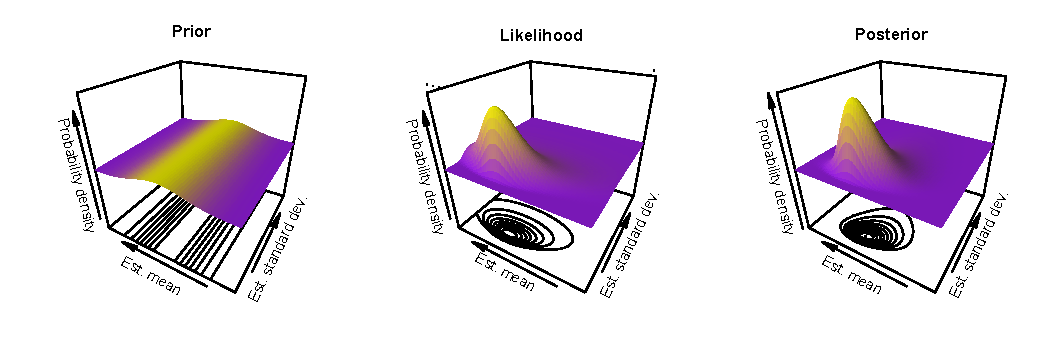
\includegraphics[width=1.4\textwidth]{multiparameter_bayes.pdf}}
\caption{Multiparameter Bayesian inference.}
\label{fig:multiparameter_bayes}
\end{figure}

In summary, shifting from classical methods to Bayesian ones would make statistics within DCA more transparent to both its engineers and clients. Hypothesis tests and interval estimates are easily misinterpreted and needlessly obscure the amount of certainty in parameter estimates. The jargon of classical statistics can make it unclear what's relevant to the problem at hand, and makes an honest explanation of its methods to non-technical team members difficult and comical. Bayesian methods make it clear how the data and prior knowledge are being combined, and provide results that are more easily interpreted.
\par
It is generally recognized that the scientific community as a whole needs to reconsider the practical relevance of hypothesis testing: DCA can hardly be faulted for neglecting to apply ineffective methods.

\subsection*{Markov Chain Monte Carlo}
As mentioned, DCA have previously used Monte Carlo simulation to approximate the distribution of a tolerance chain's dimension. For problems with many parameters - such as a subassembly of many components - Monte Carlo simulation isn't feasible because it would require an outrageous number of grid points. Instead, the posterior can be approximated using a Markov chain Monte Carlo method. This entails randomly drawing a sequence of values according to their relative probabilities, such that their relative frequencies reflect the posterior distribution.

%%
\section{Presentation \& Visualization}
\subsection{The Psychology of a Plot}
\subsection{Scatter plots}
\subsection{Box plots}
\subsection{Separation Plots}
http://mdwardlab.com/sites/default/files/GreenhillWardSacks.pdf

%%
\section{Software}
\begin{itemize}
\item Excel
\item Matlab
\item R
\item Python
\item Minitab
\end{itemize}

\newpage


%% CONCLUSIONS AND RECOMMENDATIONS %%
\chapter{Conclusions \& Recommendations}

\newpage
\appendix
\chapter{}
Probability allows us to analyze a system without requiring complete mechanical knowledge of it. `'Randomness'' refers to sources of variation that aren't measured. You may have heard of probabilities as representing `'Degrees of belief''. To understand what a belief is, consider this example. We machine a coin that we check is a symmetric disk of homogeneous density. I flip the coin ten times, and it comes up heads every single time. You might be surprised by this, and accuse me of flipping it in a controlled way. I then ask you how I can flip it in a way that is fair. What is your response?
\par
If you say that it should come heads as many times as tails, then the experiment is no longer random, as we know what the outcome will be. You may gesticulate and say ``You need to flip it \emph{randomly}''. I would press you to tell me what this means - I require a mechanism to decide how to flip the coin, and physical mechanisms are deterministic.
\par
The probability of an outcome can only be evaluated relative to a set of assumptions you make about the mechanism generating those outcomes. You had a preconceived notion that the way I flipped the coin would favor neither heads nor tails, and therefore saw ten heads as supremely improbable.
\newpage
We can see this by recognizing that the sum of independent observation's variances is equal to the variance of the variance of the sum of the observations:
\begin{align}
 \text{Var}\sum_{i = 1}^n X_i &= \sum_{i = 1}^n \text{Var}X_i\\
	\text{Var}n\bar{X} &= n\text{Var}X \\
	\implies \sqrt{\text{Var}\bar{X}} &= \frac{\sigma}{\sqrt{n}}
\end{align}
\par
Analytically, we can solve for $p(\theta|y)$ directly
\[
  p(\theta|y) \propto \binom{n}{y}\theta^y (1 - \theta)^{n-y}\cdot 1
\]
To find the constant of proportionality, we need to divide the r.h.s. by its integral over all values of $\theta$, such that the $\int_0^1 p(\theta|y)\cdot d\theta = 1$. As it happens, the r.h.s. has the form of what's called a beta distribution
\[
  p(x; a, b) \propto x^{a - 1}\cdot x^{b-1}
\]

Confidence intervals
\[
	 = \text{P}\Bigg(\frac{\Big(\frac{\bar{x} - \mu}{\sigma/\sqrt{n}}\Big)}{s/\sqrt{n}\sigma}\Bigg)
\]
\end{document}